\chapter{El algoritmo CORDIC}
\label{cap:apC}

A continuación se detalla el fundamento matemático del algoritmo.

Sea un vector $\textbf{x}=(x,y)$ perteneciente al plano y una rotación del mismo $\mathbf{x}_{\phi}=(x_{\phi},y_{\phi})$
en un ángulo $\phi$, los cuales se observan en la Fig. \ref{vectorrotacion}.

\begin{figure}[htpb]
\begin{center}
\scalebox{1}{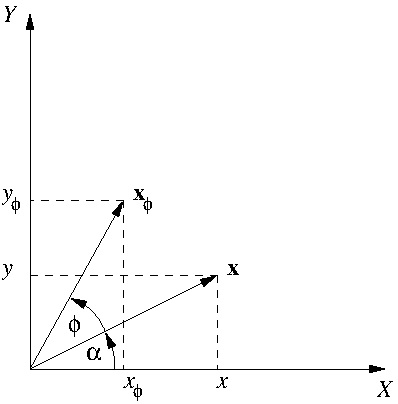
\includegraphics[angle = 0]{./figures/APC-figura_1.pdf}}
\caption{Rotación de un vector en un ángulo $\phi$.}
\label{vectorrotacion}
\end{center}
\end{figure}

Si $\textbf{x}$ posee norma unitaria, $\|\mathbf{x}\|=1$, se cumple

\begin{equation}
\begin{array}{l}
x=\cos(\alpha)\\
\\
y=\sin(\alpha)\\
\end{array}
\end{equation}

Dadas las siguientes identidades trigonométricas 

\begin{equation}
\begin{array}{l}
\sin(\alpha+\beta)=\sin(\alpha)\cos(\beta)+\cos(\alpha)\sin(\beta)\\
\\
\cos(\alpha+\beta)=\cos(\alpha)\cos(\beta)-\sin(\alpha)\sin(\beta)\\
\end{array}
\end{equation}

resulta

\begin{equation}
\label{ec1}
\begin{array}{l}
x_{\phi}=\cos(\alpha+\phi)=\cos(\alpha)\cos(\phi)-\sin(\alpha)\sin(\phi)=x\cos(\phi)-y\sin(\phi)\\
\\
y_{\phi}=\sin(\alpha+\phi)=\sin(\alpha)\cos(\phi)+\cos(\alpha)\sin(\phi)=y\cos(\phi)+x\sin(\phi)\\
\end{array}
\end{equation}

o bien en su forma matricial equivalente:

\begin{equation}
\left[
\begin{array}{c}
x_{\phi}\\
y_{\phi}\\
\end{array}
\right]
=
\left[
\begin{array}{cc}
\cos(\phi) & \sin(\phi)\\
-\sin(\phi) & \cos(\phi)\\
\end{array}
\right]
\left[
\begin{array}{c}
x\\
y\\
\end{array}
\right]
\end{equation}

Tomando como factor común $\cos(\phi)$ en la ecuación \ref{ec1} se obtiene,

\begin{equation}
\begin{array}{l}
x_{\phi}=\cos(\phi)\lbrack x-y\tan(\phi)\rbrack\\
\\
y_{\phi}=\cos(\phi)\lbrack y+x\tan(\phi)\rbrack\\
\end{array}
\end{equation}

donde $\cos(\phi) > 0$ si $-\pi/2 < \phi < \pi/2$.

Ahora bien, si se restringe el ángulo de rotación a un conjunto discreto de valores $\phi_{i}$ de forma tal que su
tangente tome los valores

\begin{equation}
\tan(\phi_{i})=2^{-i}, \quad	i=0,1,2,\ldots,n-1; \quad n \in \mathbb N 
\end{equation}

entonces

\begin{equation}
\label{ec3}
\begin{array}{l}
x_{i+1}=k_{i} \left[ x_{i}-y_{i} d_{i} 2^{-i}   \right]\\
\\
y_{i+1}=k_{i} \left[ y_{i}+x_{i} d_{i} 2^{-i}   \right]\\
\end{array}
\end{equation}

donde

\begin{equation}
\label{ec2}
k_{i}=\cos(\phi_{i})=\displaystyle \frac{1}{\sqrt{1+2^{-2i}}}
\end{equation}

y $d_{i}$ sólo puede adoptar los valores $+1$ ó $-1$.

\emph{Demostración de la ecuación \ref{ec2}:}

Si $\phi \ne \pm \pi/2$ entonces,

\begin{equation}
\label{eca1}
\tan{(\phi_i)}=\frac{\sin{(\phi_i)}}{\cos{(\phi_i)}}
\end{equation}

Restringiendo $\phi_i$ de forma tal que sólo acepte aquellos valores para los cuales su tangente corresponde a potencias enteras negativas de 2, es decir $\tan(\phi_i)=2^{-i}$ y elevando al cuadrado la ecuación (\ref{eca1}) se obtiene

\begin{equation}
\tan^2{(\phi_i)}=2^{-2i}=\frac{\sin^2{(\phi_i)}}{\cos^2{(\phi_i)}}
\end{equation}

Siendo $\cos^2{(\phi_i)} + \sin^2{(\phi_i)} = 1$, se cumple

\begin{equation}
2^{-2i}=\frac{1-\cos^2{(\phi_i)}}{\cos^2{(\phi_i)}}=\frac{1}{\cos^2{(\phi_i)}}-1
\end{equation}

y por lo tanto

\begin{equation}
1+2^{-2i}=\frac{1}{\cos^2{(\phi_i)}}
\end{equation}

Por último,

\begin{equation}
k_i=\cos{(\phi_i)}=\frac{1}{\sqrt{1+2^{-2i}}}
\end{equation}

Si se realizan $n$ rotaciones sucesivas sobre un vector $\mathbf{x_{0}}=\left[ x_{0} \ y_{0} \right] ^T \in
\mathbf{R}^2$, se obtiene,

\begin{equation}
\begin{array}{l}
x_{n} = x_0 \cos \left( \sum_{i=0}^{n-1}{d_{i}\arctan \left( 2^{-i} \right)  } \right) - y_0 \sin \left( \sum_{i=0}^{n-1}
{d_{i}\arctan \left( 2^{-i} \right)  } \right) \\
\\
y_{n}=x_0 \sin \left( \sum_{i=0}^{n-1}{d_{i}\arctan \left( 2^{-i} \right)  } \right) -y_0 \cos \left( \sum_{i=0}^{n-1}
{d_{i}\arctan \left( 2^{-i} \right)  } \right) \\
\end{array}
\end{equation}

Por lo tanto, si se realiza una rotación en un ángulo $\phi$, el ángulo verdadero de rotación obtenido luego de $n$
iteraciones será

\begin{equation}
\label{ec5}
\phi_{n}=\sum_{i=0}^{n-1} d_{i} \arctan \left( 2^{-i} \right)
\end{equation}

Las siguientes definiciones son ahora necesarias:

\begin{defi}
Se define como error $\mathbf{\epsilon_x}$ entre una magnitud $x$ y una aproximación $\hat{x}$ de la misma a la
diferencia $\epsilon_x=x-\hat{x}$.
\end{defi}

\begin{defi}
Se define como error absoluto $e_x$ entre una magnitud $x$ y una aproximación $\hat{x}$ de la misma al valor
$e_x=|\epsilon_x|=|x-\hat{x}|$.
\end{defi}

\begin{defi}
Se define como incertidumbre $\Delta x$ de una magnitud $x$ a la inferior de las cotas superiores $M$ tales que
$|x-\hat{x}|\le M$.
\end{defi}

Con estas definiciones en mente, se puede escribir

\begin{equation}
\label{ec11}
e_{\phi}=|\phi - \phi_{n}| \le \displaystyle \frac{1}{2} \arctan \left( 2^{-n+1} \right) =\Delta \phi
\end{equation}

con lo cual probarse que

\begin{equation}
\lim_{n \to \infty}e_{\phi} = 0
\end{equation}

En la Fig. \ref{error} se observa $\Delta \phi$ en función de la cantidad de iteraciones $n$.

\begin{figure}[htpb]
\begin{center}
\scalebox{0.7}{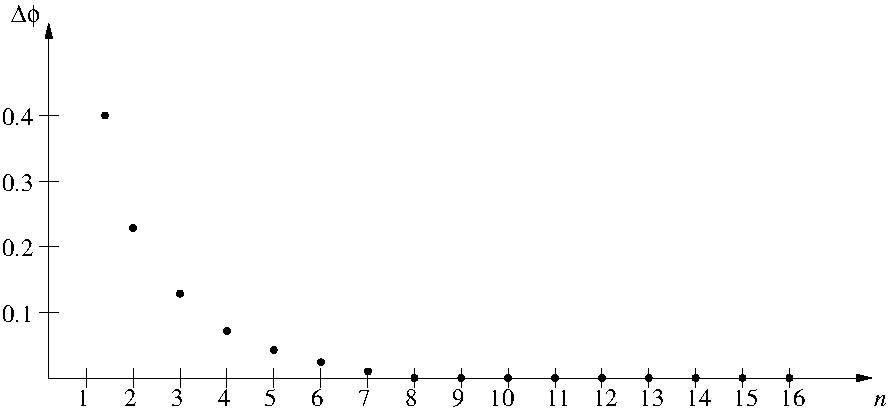
\includegraphics[angle = 0]{./figures/APC-figura_2.pdf}}
\caption{$\Delta \phi$ en función de la cantidad de iteraciones $n$.}
\label{error}
\end{center}
\end{figure}

Por otra parte, definiendo

\begin{equation}
\label{ec4}
\begin{array}{l}
x_{i+1}'=x_{i}'-y_{i}' d_{i} 2^{-i}\\
\\
y_{i+1}'=y_{i}'+x_{i}' d_{i} 2^{-i}\\
\\
\end{array}
\end{equation}

donde $i=0,1, \ldots, n-1$, se observa a partir de la ecuación \ref{ec3} que

\begin{equation}
\begin{array}{lll}
x_{i+1} & = & k_{i}\left(x_{i}-y_{i}d_{i}2^{-i}\right)\\
\\
        & = & k_{i}\left[ k_{i-1}\left(x_{i-1}-y_{i-1}d_{i-1}2^{-i+1}\right) - k_{i-1}\left(y_{i-1}+
x_{i-1}d_{i-1}2^{-i+1}\right)d_{i} 2^{-i} \right]\\
\\
        & = & k_{i}k_{i-1}\left(x_{i}'-y_{i}'d_{i}'2^{-i}\right)\\
\\
\\
y_{i+1} & = & k_{i}\left(y_{i}+x_{i}d_{i}2^{-i}\right)\\
\\
        & = & k_{i}\left[ k_{i-1}\left(y_{i-1}+x_{i-1}d_{i-1}2^{-i+1}\right) +
 k_{i-1}\left(x_{i-1}-y_{i-1}d_{i-1}2^{-i+1}\right)d_{i} 2^{-i} \right]\\
\\
        & = & k_{i}k_{i-1}\left(y_{i}'+x_{i}'d_{i}'2^{-i}\right)\\
\end{array}
\end{equation}

y por lo tanto

\begin{equation}
\begin{array}{l}
x_{n}=\left(\prod_{i=0}^{n-1}k_{i}\right)x_{n}'\\
\\
y_{n}=\left(\prod_{i=0}^{n-1}k_{i}\right)y_{n}'\\
\end{array}
\end{equation}

se concluye que resulta conveniente realizar la iteración mediante la ecuación (\ref{ec4}), obteniendo los valores de
$x_{n}'$ y $y_{n}'$. Luego los valores de $x_{n}$ y $y_{n}$ pueden hallarse mediante el producto por $k_{n}$,

\begin{equation}
\begin{array}{l}
x_{n}=k_{n} x_{n}'\\
\\
y_{n}=k_{n} y_{n}'\\
\end{array}
\end{equation}

donde $k_{n}$ corresponde a la constante dada por:

\begin{equation}\label{eckn}
k_{n}= \prod_{i=0}^{n-1}k_{i}=\prod_{i=0}^{n-1} \displaystyle \frac{1}{\sqrt{1+2^{-2i}}}
\end{equation}

La ecuación (\ref{ec4}) define el algoritmo CORDIC y provee un método para hallar las componentes $x_{n}'$, $y_{n}'$
sin el uso de productos matriciales, sólo mediante operaciones de suma, resta y desplazamiento como se detallará más
adelante. Los dos valores $x_{n}'$, $y_{n}'$ corresponden a las componentes del vector $\mathbf{x}$ rotado un ángulo
$\phi_{n}$ dado por la ecuación (\ref{ec5}) y escalado por un valor $A_{n}=1/k_{n}$ conocido como \emph{ganancia de procesamiento}.

En la figura \ref{pseudorotacion} se observa el efecto de alargamiento del vector en cada iteración del algoritmo, por
lo que cada una de estas es a menudo llamada \emph{pseudorotación}, ya que no conserva la norma.

\begin{figure}[htpb]
\begin{center}
\scalebox{0.7}{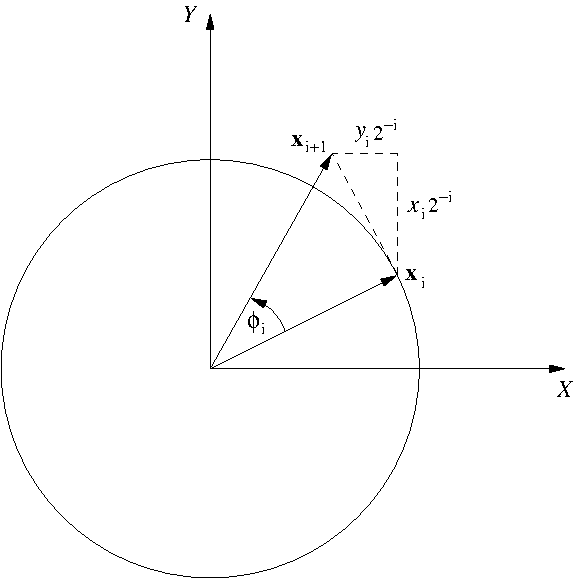
\includegraphics[angle = 0]{./figures/APC-figura_4.pdf}}
\caption{Pseudorotación producida por la \emph{i}-ésima iteración.}
\label{pseudorotacion}
\end{center}
\end{figure}

Por último, si para una rotación dada no se conoce la secuencia de valores $\left\{d_{i}\right\}_{i=0,1, \ldots ,n-1}$,
entonces se utiliza un acumulador de fase $z_{i}$ donde deben conocerse todos los valores $\arctan\left( 2^{-i} \right)$
para $i=0,1, \ldots, n-1$;

\begin{equation}
\begin{array}{l}
z_{i+1}=z_i-d_i\arctan \left( 2^{-i} \right)\\
\\
d_i=\left\{ 
	\begin{array}{ll}
	-1 & \mbox{si } z_{i} < 0,\\
	+1 & \mbox{si } z_{i} \ge 0.
	\end{array} \right.
\end{array}
\end{equation}

\section{Convergencia del algoritmo CORDIC}

Para asegurar la convergencia del algoritmo luego de infinitas iteraciones debe asegurarse que el vector resultante
converja en fase, es decir el ángulo $\phi_n$ se aproxima tanto como se desee al ángulo $\phi$, y además la que converja
en norma, lo que implica que el factor de escala $A_{n}$ debe ser finito cuando $n$ tiende a infinito.

La ecuación (\ref{ec11}) muestra la convergencia del algoritmo respecto del ángulo de rotación debido a la monotonicidad
creciente de la función arcotangente y la monotonicidad decreciente de su argumento $2^{-N+1}$.

\subsection{Convergencia en norma}
Luego de $n$ iteraciones, ambas salidas del algoritmo CORDIC se ven escaladas por un
factor

\begin{equation}
A_{n}=\prod_{i=0}^{n-1}\sqrt{1+2^{-2i}}= \sqrt{\prod_{i=0}^{n-1} \left(1+2^{-2i}\right)}
\end{equation}

Para probar la convergencia de $A_{n}$, alcanza encontrar una cota superior y una cota inferior. Una cota inferior es
simple de encontrar, ya que $A_{n}$
corresponde a la productoria de factores todos ellos positivos independientemente del valor de $i$, por lo tanto
$A_{n}\geq 0$, $\forall n \in \mathbf{N}$.

Para encontrar una cota superior se analizan los términos parciales de la sucesión $\left\{\prod_{i=0}^{n-1}
\left(1+2^{-2i}\right)\right\}_{n \in \mathbf{N}}$.

\begin{enumerate}

\item $n=0$

\hspace{1cm}
\begin{math}
\displaystyle\prod_{i=0}^{n-1} 1+2^{-2i}=1+2^0=2
\end{math}


\item $n=1$

\hspace{1cm}
\begin{math}
\displaystyle\prod_{i=0}^{n-1} 1+2^{-2i}=2\left(1+2^{-2}\right)=2+2^{-1}
\end{math}


\item $n=2$

\hspace{1cm}
\begin{math}
\displaystyle\prod_{i=0}^{n-1} 1+2^{-2i}=\left(2+2^{-1}\right)
\left(1+2^{-4}\right)=2+2^{-1}+2^{-3}+2^{-5}
\end{math}


\item $n=3$

\hspace{1cm}
\begin{math}
\begin{array}{lll}
\displaystyle\prod_{i=0}^{n-1} 1+2^{-2i} & = & \left(2+2^{-1}+2^{-3}+2^{-5}\right) \left(1+2^{-6}\right)\\
							& = & 2+2^{-1}+2^{-3}+2^{-4}+2^{-7}+2^{-9}+2^{-11}\\
\end{array}
\end{math}


\item $n=4$

\hspace{1cm}
\begin{math}
\begin{array}{lll}
\displaystyle\prod_{i=0}^{n-1}
1+2^{-2i} & = & \left(2+2^{-1}+2^{-3}+2^{-4}+2^{-7}+2^{-9}+2^{-11}\right) \left(1+2^{-8}\right)\\
          & = & 2+2^{-1}+2^{-3}+2^{-4}+2^{-6}+2^{-8}+2^{-10}+2^{-12}+2^{-15}\\
		  &   & +2^{-17}+2^{-19}\\
\end{array}
\end{math}


\item $n=5$

\hspace{1cm}
\begin{math}
\begin{array}{lll}
\displaystyle\prod_{i=0}^{n-1}1+2^{-2i} & = & (2+2^{-1}+2^{-3}+2^{-4}+2^{-6}+2^{-8}+2^{-10}+2^{-12}+2^{-15}\\
		  			&   & +2^{-17}+2^{-19}) \left(1+2^{-10}\right)\\
		  	\\
		           & = & 2+2^{-1}+2^{-3}+2^{-4}+2^{-6}+2^{-8}+2^{-9}+2^{-10}+2^{-11}\\
                           &   & +2^{-12}+2^{-14}+2^{-15} +2^{-16}+2^{-17}+2^{-18}+2^{-19}\\
                           &   & +2^{-20}+2^{-22}+2^{-25}+2^{-27}+2^{-29}\\
\end{array}
\end{math}

\end{enumerate}

Se observa que el término de mayor orden corresponde a $2^{-\left(n^2+n-1 \right)}$. Si
bien no están presentes todos los términos hasta $2^{-\left(n^2+n-1 \right)}$, se
puede ver que 

\begin{equation}
\prod_{i=0}^{n-1} 1+2^{-2i}<1+\sum_{i=0}^{k}2^{-i}<1+\sum_{i=0}^{\infty}2^{-i}=3, \quad k=n^2+n-1
\end{equation}

Por lo tanto,

\begin{equation}
A_{n}=\prod_{i=0}^{n-1}\sqrt{1+2^{-2i}}<\sqrt{3}\cong 1.73205
\end{equation}

De esta forma se concluye que el algoritmo CORDIC converge luego de infinitas
iteraciones alcanzando un error nulo en el ángulo de rotación y un factor de escala $A_{n} \cong 1,64676$.

Si se desean los valores de $x_{n}$ y $y_{n}$ sin el factor de escala, se puede multiplicar la salida del algoritmo,
$x_{n}'$, $y_{n}'$ por $k_{n}=1/A_{n}$, el cual adquiere un valor de aproximadamente $0.60725$ logrando así que el
algoritmo conserve la norma original del vector de entrada $\mathbf{x}_0$.

Estas observaciones son formalizadas a continuación. A partir de (\ref{eckn}) se define

\begin{equation}\label{exkn2}
k_n^2=\prod_{i=0}^{n-1}{\frac{1}{1+2^{-2i}}}
\end{equation}

\begin{prop}
La suceción $\left\{k_n^2\right\}_{n\in\mathbf{N}}$ es una sucesión decrecientes de números reales positivos.
\end{prop}

\emph{Demostración:}

Para demostrar que cada término de la sucesión es positivo basta observar que cada factor de la productoria definida en
 (\ref{exkn2}) es positivo y para demostrar que es decreciente basta observar a su vez que cada factor es menor a 1.

\

Estas dos observaciones implica que la sucesión $\left\{k_n^2\right\}_{n\in\mathbf{N}}$ está acotada inferiormente con
lo cual es convergente y entonces se puede enunciar el siguiente teorema.

\begin{teor}
La suceción $\left\{k_n^2\right\}_{n\in\mathbf{N}}$ converge en $\mathbf{R}$. Aún más, converge a un número mayor a cero.
\end{teor}

\emph{Demostración:}

Al ser una sucesión monótonamente decreciente y acotada inferiormente por cero necesariamente converge por la
completitud de $\mathbf{R}$.

La convergencia a un número mayor a cero se hará por el absurdo. Sunpóngase que efectivamente
$\left\{k_n^2\right\}_{n\in\mathbf{N}}$ converge a 0. Entonces por definición de convergencia, para todo
$\varepsilon >0$ existe $N \in \mathbf{N}$ tal que si $n\geq N$ se cumple $|k_n^2-0|=k_n^2<\varepsilon$. Por lo tanto,

\begin{equation}
\prod_{i=0}^{n-1}{\frac{1}{1+2^{-2i}}}<\varepsilon
\end{equation}

Lo cual se cumple si y sólo si

\begin{equation}\label{dsfsdf}
1 < \varepsilon \prod_{i=0}^{n-1}{1+2^{-2i}} \qquad \forall \varepsilon > 0
\end{equation}

Sea $0 < \varepsilon = 1/(2\prod_{i=0}^{n-1}{1+2^{-2i}})$ entonces resulta de la ecuación  \ref{dsfsdf} que $1<1/2$ lo
cual es absurdo y parte de suponer que $\left\{k_n^2\right\}_{n\in\mathbf{N}}$ converge a 0.

\

De esta forma se concluye que si $\left\{k_n^2\right\}_{n\in\mathbf{N}}$ converge entonces también lo hace
$\left\{k_n\right\}_{n\in\mathbf{N}}$ y en consecuencia $\left\{A_n\right\}_{n\in\mathbf{N}}$. Por lo que queda demostrada la convergencia en norma del algoritmo.

\subsection{Convergencia en fase}

La convergencia en fase se demuestra haciendo uso del llamado \emph{Teorema de Convergencia}:

\begin{teor}
Sea $\{ \sigma_0, \, \sigma_1 , \,\ldots , \,\sigma_{n}\}$ una secesión finita decreciente de $n+1$ números positivos,
es decir $\sigma_i \ge \sigma_j$ para $i \ge j$, la cual cumple que

\begin{equation}
\sigma_k \le \sigma_{n} + \sum_{j=k+1}^{n}{\sigma_j}, \quad 0 \le k \le n
\end{equation}

Además, sea $r$ un número positvo que satisface

\begin{equation}
|r| \le \sum_{j=0}^{n}{\sigma_j}
\end{equation}

Sea también la sucesión $s_0=0$, $s_{k+1}=s_k + \delta_k\sigma_k$, $k=0,1,\ldots,n$, donde

\begin{equation}
\delta_k=sgn(r-s_k)=\left\{\begin{array}{rcl}
				1, & r \ge s_k\\
				-1, & r \le s_k\\
			\end{array}\right.
\end{equation}

Entonces,

\begin{equation}
|r-s_k| \le \sigma_{n} + \sum_{j=k}^{n}{\sigma_j}, \quad 0 \le k \le n
\end{equation}

En particular,

\begin{equation}
|r-s_{n+1}| \le \sigma_{n}
\end{equation}

\end{teor}

\emph{Demostración:}

La demostración se realizará por inducción sobre $k$. Para $k=0$, se tiene

\begin{equation*}
|r-s_0|=|r| \le \sigma_{n}+\sum_{j=0}^{n}{\sigma_j}
\end{equation*}

Asumiendo el teorema válido para $k$, se tiene la siguiente hipótesis inductiva (H1)

\begin{equation*}
|r-s_k| \le \sigma_{n} + \sum_{j=k+1}^{n}{\sigma_j}
\end{equation*}

Considerando el caso $k+1$, se debe demostrar que la siguiente tesis inductiva (T1) es válida

\begin{equation*}
|r-s_{k+1}| \le \sigma_{n} + \sum_{j=k+1}^{n}{\sigma_j}
\end{equation*}

Considérese $|r-s_{k+1}|= |r-s_k-\delta_k\sigma_k|$. Si $r-s_k \ge 0$, entonces $\delta_k=1$ y
$|r-s_k-\delta_k\sigma_k|=||r-s_k|-\sigma_k|$. Por el contrario, si $r-s_k < 0$, entonces $\delta_k=-1$ y
$|r-s_k-\delta_k\sigma_k|=|r-s_k+\sigma_k|=||r-s_k|-\sigma_k|$. Por lo tanto, en ambos casos

\begin{equation*}
|r-s_{k+1}|=||r-s_k|-\sigma_k| \le \sigma_{n} + \sum_{j=k+1}^{n}{\sigma_j}
\end{equation*}

Lo que muestra que la tésis inductiva T1 es válida. Finalmente,
$-\sigma_n \le \|r-s_n\| - \sigma_n \le 2 \sigma_n-\sigma_n=\sigma_n$ y entonces
$|r-s_{n+1}|=| |r-s_n| - \sigma_n|\le \sigma_n$, lo cual completa la demostración.

\

\begin{teor}
Para $n>3$, la sucesión $\sigma_{k}=\arctan\left(2^{-k}\right)$, $k=0,1,\ldots,n$ satisface las hipótesis del teorema de
convergencia para todo $|r| \le \pi/2$.
\end{teor}

\emph{Demostración:}

La secuencia $\arctan\left(2^{0}\right),\arctan\left(2^{-1}\right),\ldots,\arctan\left(2^{-n}\right)=
\arctan\left(1\right),\ldots,\arctan\left(1/2^{n}\right)$ es claramente una secuencia decreciente de valores positivos.
 El Teorema del Valor Medio establece que existe un número $c$ entre $a$ y $b$, $a<c<b$, tal que

\begin{equation}\label{asdfasdf}
\frac{\arctan{(b)}-\arctan{(a)}}{b-a}=\frac{1}{1+c^2}
\end{equation}

Sean $a=2^{-(j+1)}$, $b=2^{-j}$ en (\ref{asdfasdf}). Entonces, $b-a=2^{-(j+1)}$ y además

\begin{equation}
\frac{1}{1+c^2}<\frac{1}{1+a^2}=\frac{1}{1+2^{-2(j+1)}}=\frac{2^{2j+2}}{1+2^{2j+2}}
\end{equation}

Entonces,

\begin{equation}\label{ec32}
\sigma_j-\sigma_{j+1}<(b-a)\frac{1}{1+c^2} \le \frac{1}{2^{j+1}}\frac{2^{2j+2}}{1+2^{2j+2}}=\frac{2^{j+1}}{1+2^{2j+1}}
\end{equation}

Sean ahora $a=0$, $b=2^{-j}$ en (\ref{asdfasdf}). Entonces,

\begin{equation}
\frac{1}{1+c^2}>\frac{1}{1+b^2}=\frac{1}{1+2^{-2j}}=\frac{2^{2j}}{1+2^{2j}}
\end{equation}

y

\begin{equation}
\sigma_j=b\frac{1}{1+c^2}\ge\frac{1}{2^j}\frac{2^{2j}}{1+2^{2j}}=\frac{2^j}{1+2^{2j}}
\end{equation}

Por otra parte,

\begin{equation}\label{ec35}
\sigma_k-\sigma_n=(\sigma_{k}-\sigma_{k+1})+(\sigma_{k+1}-\sigma_{k+2})+\ldots+(\sigma_{n-1}-\sigma_{n})= \sum_{j=k}^{n-1}{\sigma_j}-\sigma_{j+1}
\end{equation}

Utilizando (\ref{ec32}) en (\ref{ec35}),

\begin{equation}
\sigma_k-\sigma_n \le \sum_{j=k}^{n-1}{\frac{2^{j+1}}{1+2^{2j+2}}}=\sum_{j=k+1}^{n}{\frac{2^j}{1+2^{2j}}}\le\sum_{j=k+1}^{n}{\sigma_j}
\end{equation}

con lo cual se concluye que 

\begin{equation}
\sigma_k \le \sigma_n + \sum_{j=k+1}^{n}{\sigma_j}, \quad \forall \; 0\le k \le n
\end{equation}

Por último, como la suma de los términos $\arctan(1)$, $\arctan(1/2)$, $\arctan(1/4)$ $\arctan(1/8)$ es mayor a $\pi/2$,
entonces se concluye que

\begin{equation}
|r| \le \frac{\pi}{2}<\sum_{j=0}^{3}{\arctan{\left(2^{-j}\right)}}<\sigma_n+\sum_{j=0}^{n}{\sigma_j}
\end{equation}

lo que completa la demostración.

\

\begin{teor}
El algoritmo CORDIC converge en fase.
\end{teor}

\emph{Demostración:}

Sea la secuancia $s_k=\phi-z_k=\sum_{j=0}^{k-1}{d_j\sigma_j}$. Se observa que $s_0=\phi-z_0=0$ y
$s_{k+1}=\sum_{j=0}^{k}{d_j\sigma_j}=s_k+d_k\sigma_k$. Para $r=\phi$ se tiene
$\rho_k=\mbox{signo}(r-s_k)=\mbox{signo}(\phi-s_k)=\mbox{signo}(z_k)=d_k$. Por lo tanto, la secuancia

\begin{equation}
|\phi-s_{n+1}| \le \sigma_n = \arctan{\left(2^{-n}\right)} \le \arctan{\left(\frac{1}{2^n}\right)}
\end{equation}

satisface el Teorema de Convergencia, lo cual demuestra que el algoritmo CORDIC converge para cualquier secuencia
$\{d_i\}_{i=0,\ldots,n-1}$.